\documentclass{article}
%\usepackage[T1]{fontenc}
\usepackage{xcolor,xparse,expl3,hyperref,pdfpages,caption,fancyvrb}

% redefine \VerbatimInput
\RecustomVerbatimCommand{\VerbatimInput}{VerbatimInput}%
{fontsize=\footnotesize,
%
frame=lines,  % top and bottom rule only
framesep=2em, % separation between frame and text
rulecolor=\color{gray},
%
label=\fbox{\color{black}data.txt},
labelposition=topline,
%
commandchars=\|\(\), % escape character and argument delimiters for
% commands within the verbatim
commentchar=*        % comment character
}
                        

% Add email command
%
\ExplSyntaxOn
\NewDocumentCommand{\email}{m}
 {
  \svend_email:n { #1 }
 }
\tl_new:N \l_svend_email_tl
\seq_new:N \l_svend_email_seq
\cs_generate_variant:Nn \seq_set_split:Nnn { NnV }
\cs_new_protected:Npn \svend_email:n #1
 {
  \tl_set:Nn \l_svend_email_tl { #1 }
  \regex_replace_all:nnN { \cD. } { \c{textunderscore} } \l_svend_email_tl
  \seq_set_split:NnV \l_svend_email_seq { @ } \l_svend_email_tl
  \href{ mailto:#1 }{ \emailfont \seq_use:Nn \l_svend_email_seq { \emailat } }
 }
\ExplSyntaxOff
\newcommand\emailfont{\sffamily}
\newcommand\emailat{{\color{red}\small @}}

\title{Kocmoc SVF Eurorack Module Build Instructions for V1.6}
\author{Janne Heikkarainen (\email{janne808@radiofreerobotron.net}) \\
	}

\date{\today}

\begin{document}

\maketitle

\section{Introduction}
Kocmoc SVF module is a SSM2164 VCA chip based voltage controlled filter in Eurorack format. Kocmoc Eurorack modules are licenced under CERN Open Hardware Licence version 2 - Strongly Reciprocal licence with all rights reserved by the copyright holder. \newline

\paragraph{Kocmoc Eurorack Git repository}
\begin{flushleft}
You can find build instructions, board layouts and schematics at \newline
\end{flushleft}
\begin{center}
\href{https://www.github.com/janne808/Kocmoc-Eurorack}{https://www.github.com/janne808/Kocmoc-Eurorack}
\end{center}

\section{Theory of operation} \label{theoryofoperation}

The filter circuit is based on a classic 12dB/oct state variable filter circuit made popular by \cite{chamberlin}. The voltage control is implemented by voltage controlled amplifiers using the SSM2164 chip (or equivalent modern clone).\newline

The two voltage controlled integrators responsible for the filter operation follow the SSI2164 application note example from \cite{allaert}.

\section{Build instructions} \label{buildinstructions}

\begin{flushleft}
The PCB consists of panelized boards, one for front panel connectors and one for the power connector, integrators and input/output buffering. The boards are connected together with two 10-pin headers and a 11mm M3 PCB standoff.\newline
\end{flushleft}

\begin{flushleft}
It is important to mount the 9mm potentiometers, Thonkiconn jack sockets and the M3 board standoff first \emph{without soldering} to the control PCB and only after that attach them to the front panel with appropriate nuts.
\end{flushleft}

\begin{flushleft}
The building process should follow the following order

\begin{itemize}
\item Populate and solder resistors on both boards
\item Populate and solder diodes
\item Populate and solder capacitors on both boards
\item Populate and solder integrated circuits
\item Break the panelized boards in half and trim off mousebites
\item Solder power connector and headers (make sure the pins match from schematics and board layout)
\item Mount 11mm M3 PCB standoff with a M3 screw on the upper control board
\item Mount the snap-on 9mm Alpha potentiometers VR4 and VR1 \emph{without soldering}
\item Mount the snap-on 9mm Alpha trimmers VR3, VR5 and VR2 \emph{without soldering}
\item Mount Thonkiconn jack sockets U1, U2, U3, U4, U5 and U6 \emph{without soldering}
\item Mount the front panel
\item Fingertighten socket and potentiometer nuts to the panel
\item Solder in through-hole sockets and potentiometers
\item Tighten nuts fully
\end{itemize}
\end{flushleft}

\paragraph{SSM2164 issues}
\begin{flushleft}
The original Analog Devices SSM2164 has a fault which will burn the chip if the negative power supply rail becomes unconnected. This fault has been corrected in modern clones from SSI and Alpha but remains in Coolaudio V2164. 
\end{flushleft}

\begin{flushleft}
\cite{johnson} has researched the failure (with Oscar Salas) and proposed a fix which will be implemented in the next version of the board.
\end{flushleft}

\paragraph{Capacitors}
\begin{flushleft}
Capacitors C29 and C30 are used for compensating parasitic effects of the PCB and component leads and should be left unpopulated and populated only if needed. The parasitic effects manifest themselves as increased resonance at higher cutoff frequencies.
\end{flushleft}

\paragraph{Power connector and headers}
\begin{flushleft}
Please note that version 1.5 of the boards had their power connector and header component footprint graphics mirrored by mistake. For the header pinouts this makes no difference but confusion could arise for the power connector. In any case, if a shrouded power connector is used, it should be mounted on the bottom side of the main board with the cutout slot facing away from the board.
\end{flushleft}
\begin{flushleft}
Follow and match the board and schematic graphics to the Eurorack power connector standard to make sure the pins deliver proper voltages to the board. The board is diode protected against reverse voltage.
\end{flushleft}

\begin{thebibliography}{9}
\bibitem[Chamberlin]{chamberlin}
Hal Chamberlin.
\textit{Musical Applications of Microcomputers}.
Hayden Books, 1985.
\bibitem[Allaert]{allaert}
Jeroen Allaert.
\textit{Designing Voltage Controlled Filters for Synthesizers with the SSI2164}.
Sound Semiconductor Inc., 2019
\\\texttt{http://www.soundsemiconductor.com/downloads/AN701.pdf}
\bibitem[Johnson]{johnson}
Neil Johnson.
\textit{SSM2164/SSI2164 Information}.
Neil Johnson, 2021
\\\texttt{https://www.njohnson.co.uk/index.php?menu=2\&submenu=2\&subsubmenu=3}
\end{thebibliography}

\newpage

\appendix

\section{BOM}

\centering
\VerbatimInput[fontsize=\scriptsize, label=\fbox{\color{black}Through-hole board BOM}]{2164_svf_through-hole_bom.txt}

\newpage

\VerbatimInput[fontsize=\scriptsize, label=\fbox{\color{black}Surface mount device board BOM}]{2164_svf_smd_bom.txt}

\section{Schematics}

\centering
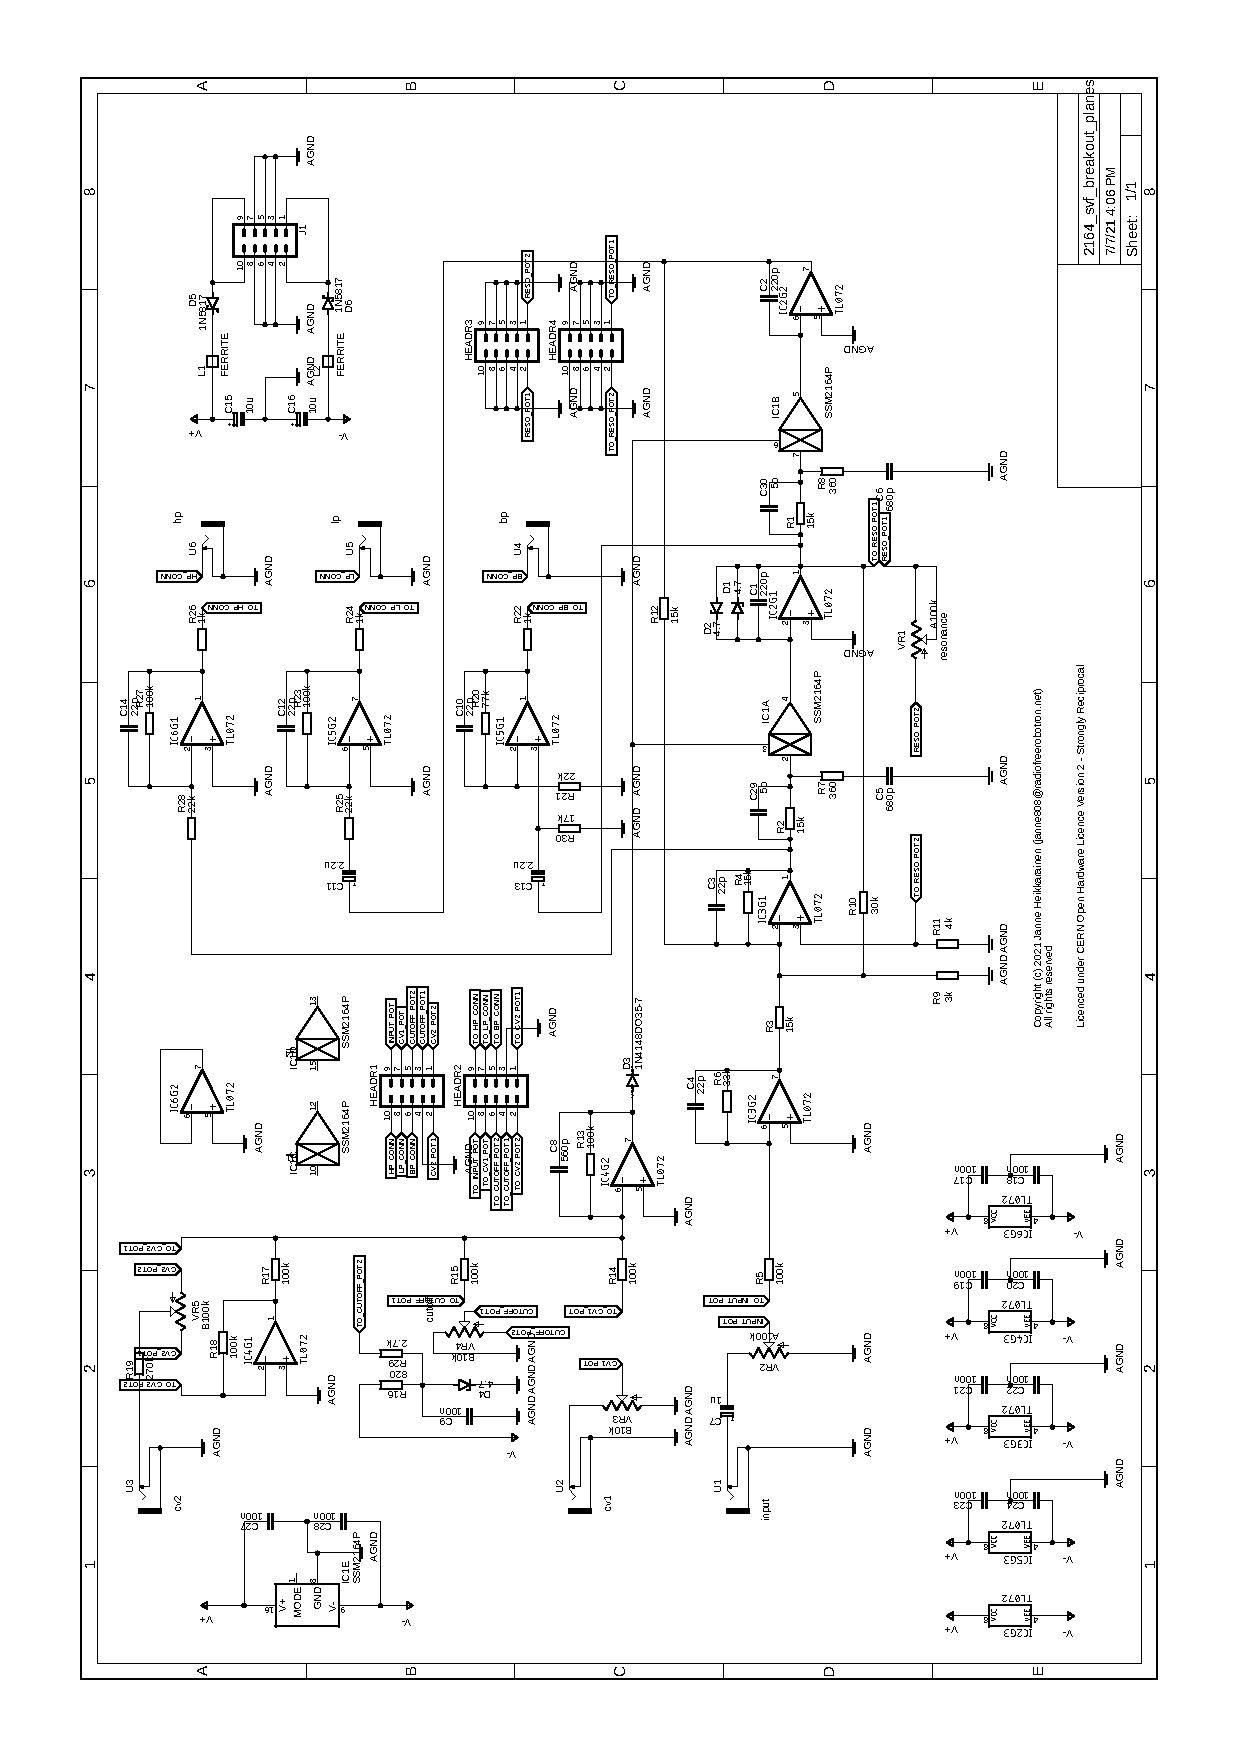
\includegraphics[page=1, scale=0.6]{2164_svf_through-hole_schematic.pdf}
\captionof{figure}{Through-hole board schematic.}

\centering
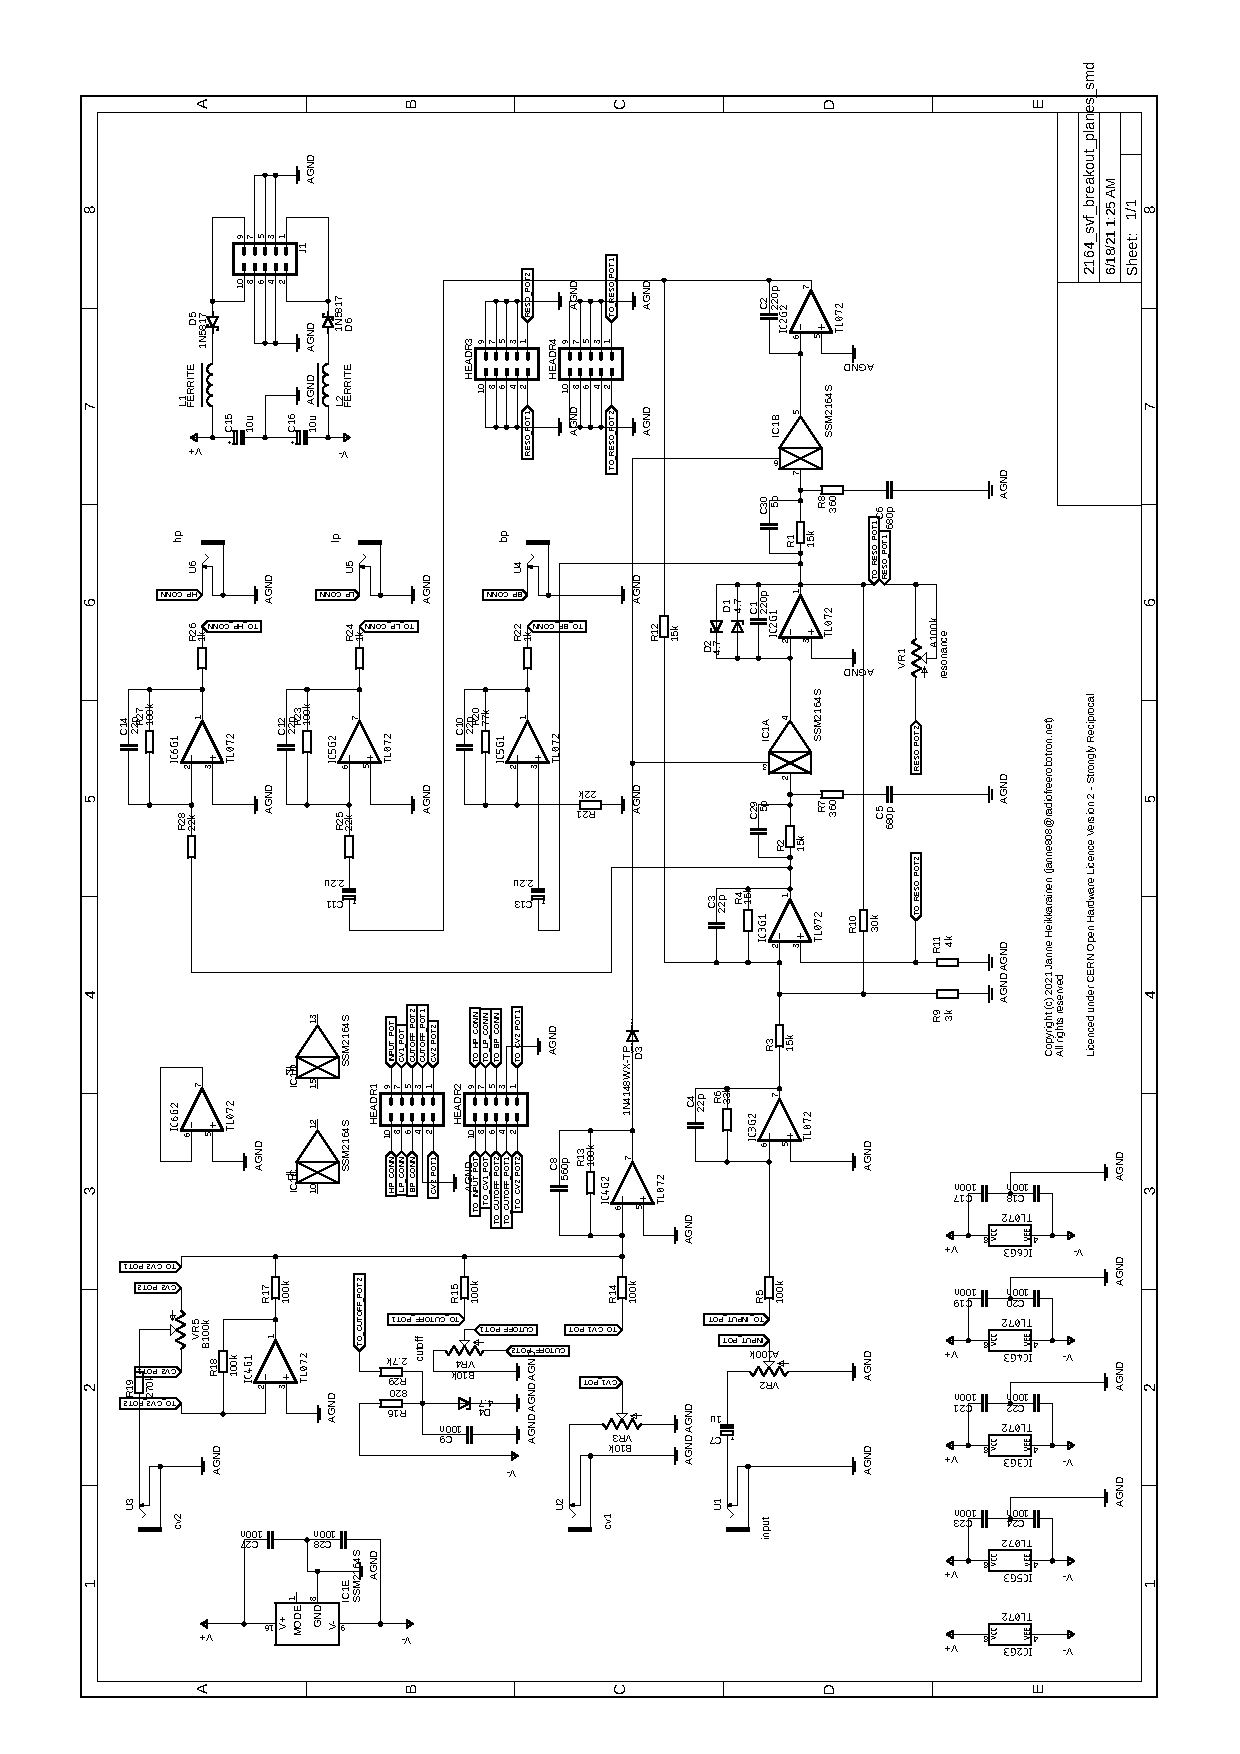
\includegraphics[page=1, scale=0.6]{2164_svf_smd_schematic.pdf}
\captionof{figure}{Surface mount device board schematic.}

\section{Board layouts}

\centering
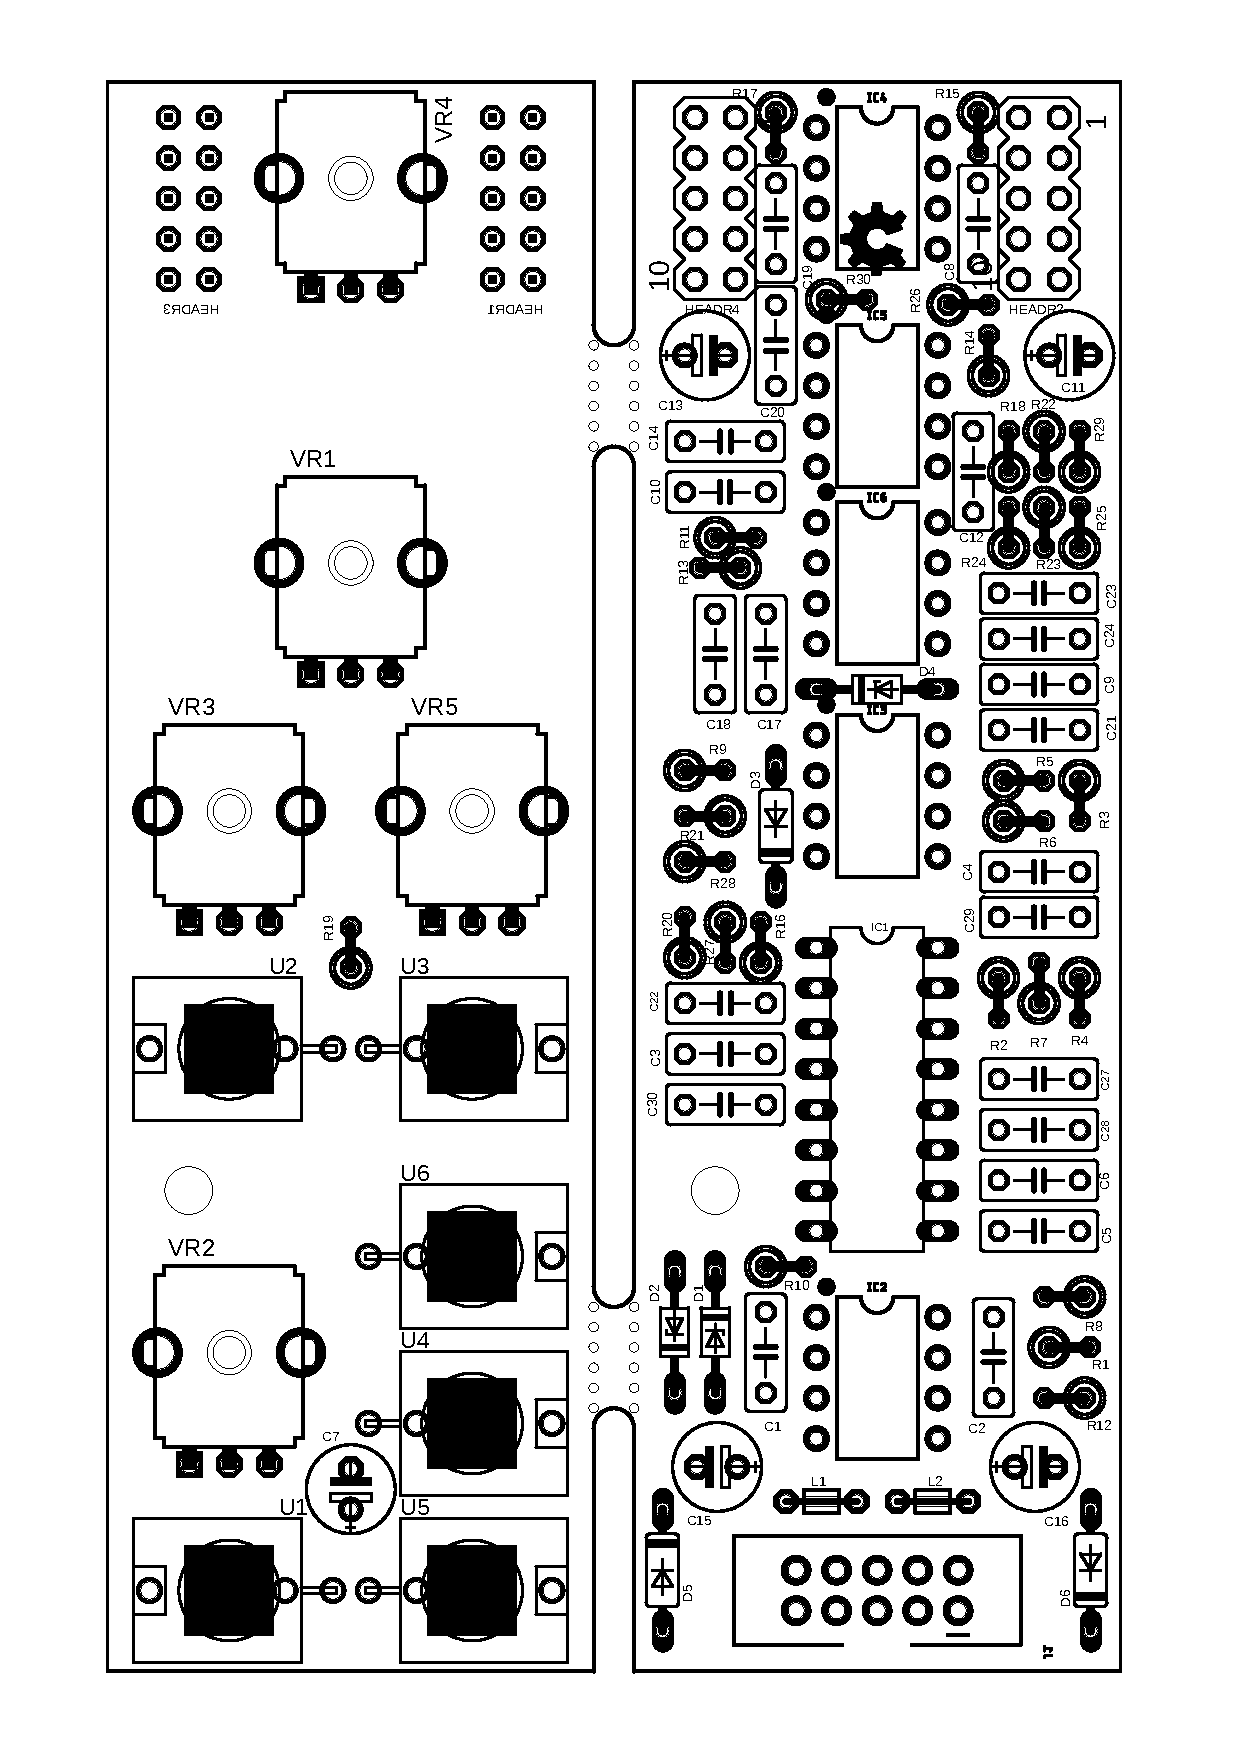
\includegraphics[page=1, scale=0.5]{2164_svf_through-hole_components.pdf}
\captionof{figure}{Through-hole board component placement for V1.6.}

\centering
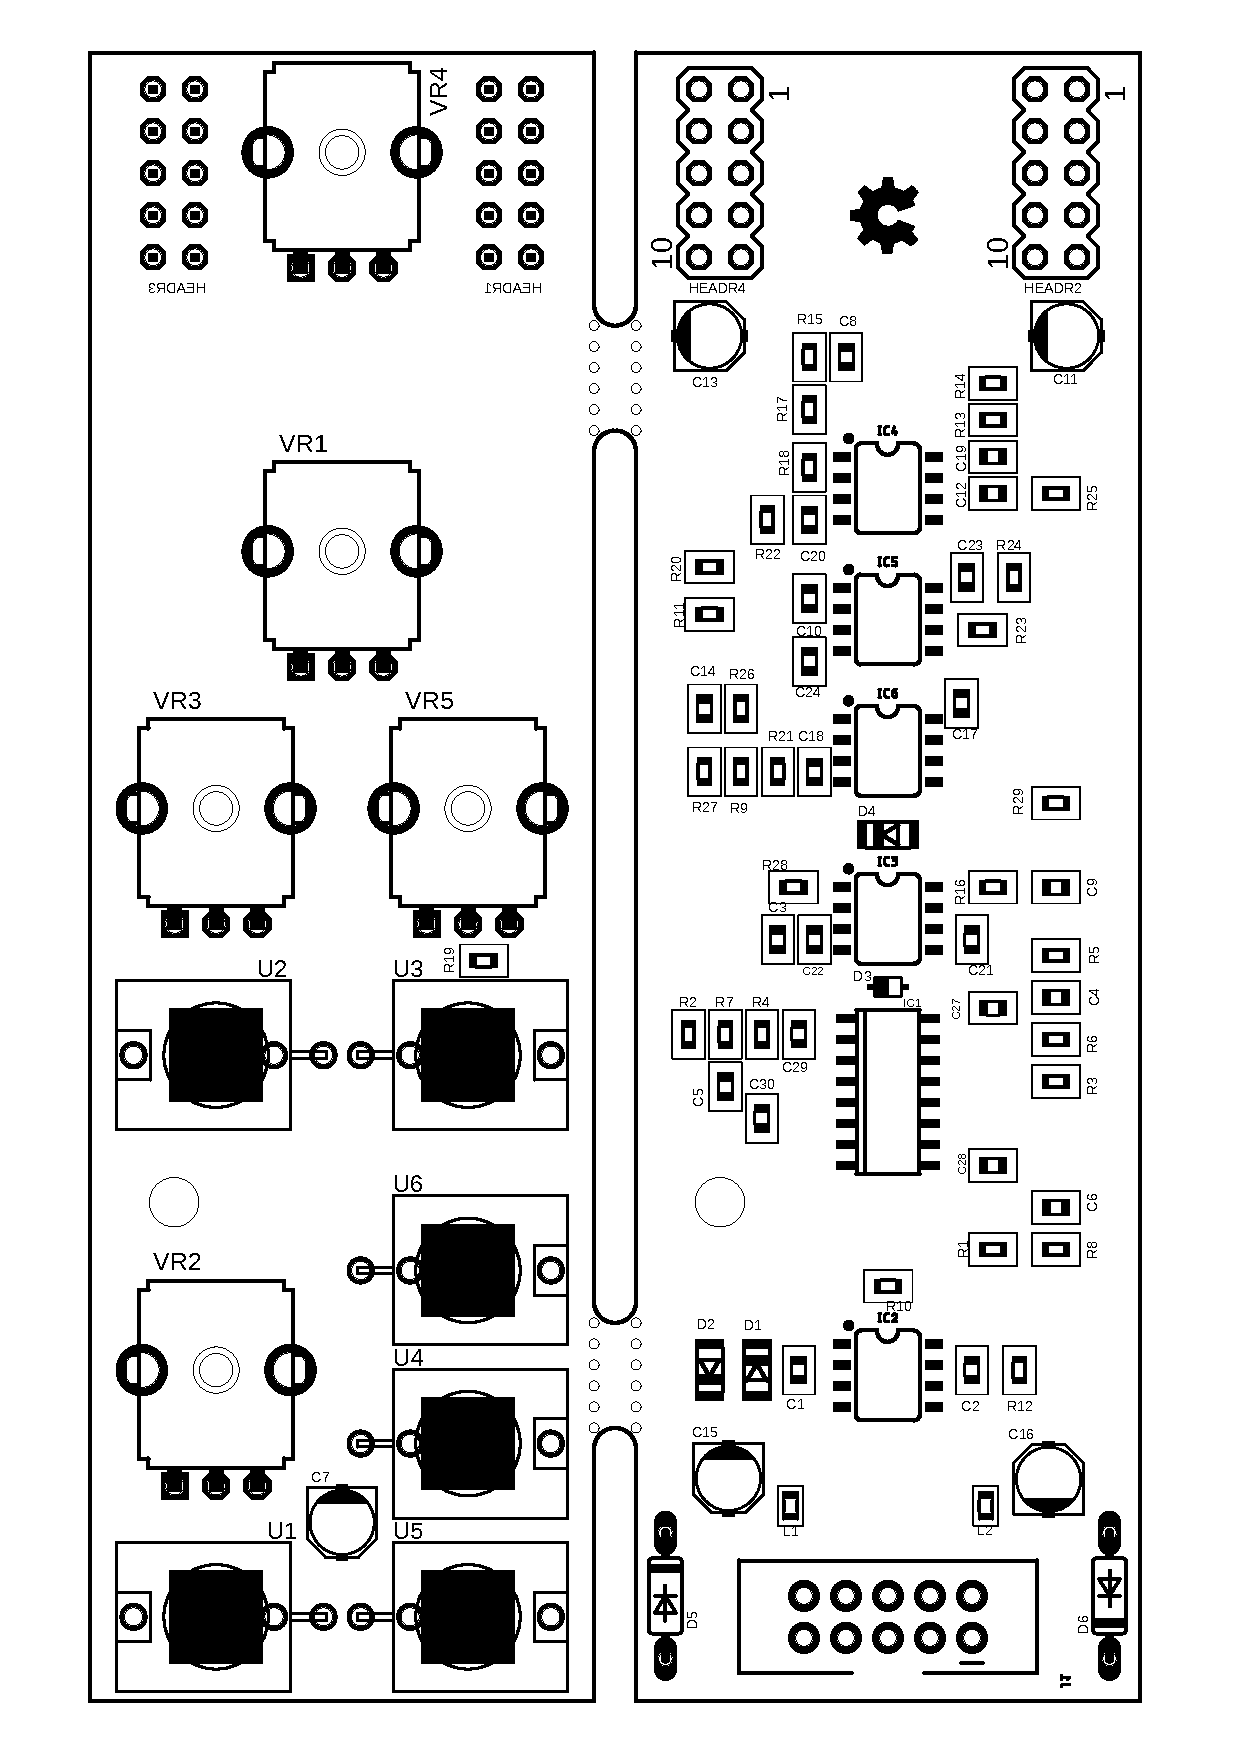
\includegraphics[page=1, scale=0.5]{2164_svf_smd_components.pdf}
\captionof{figure}{Surface mount device board component placement for V1.6.}

\end{document}

